\documentclass{standalone}
\usepackage{pgfplots}
\usepackage{xcolor}
\usepackage{libertinus}
\begin{document}
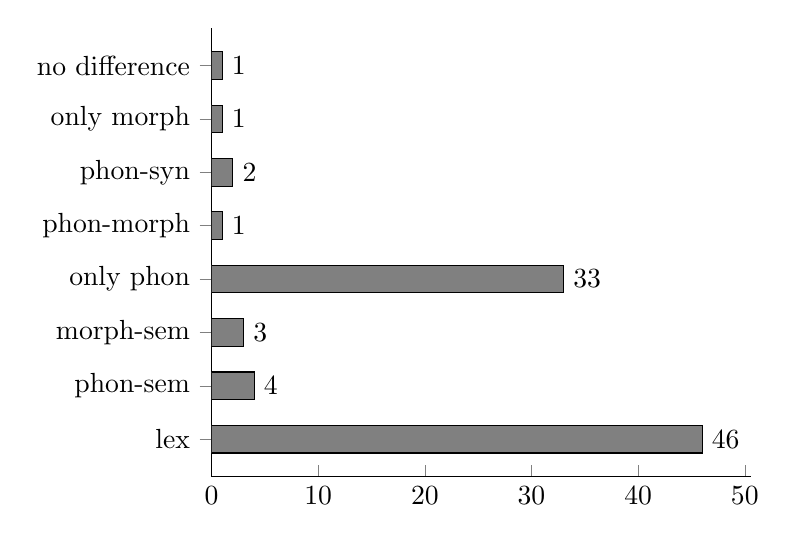
\begin{tikzpicture}
	\begin{axis}[
		xbar,
		axis lines*=left,
		symbolic y coords={lex,phon-sem,morph-sem,only phon,phon-morph,phon-syn,only morph,no difference},
		xmin = 0,
		ytick=data,
		nodes near coords,
		]
		\addplot [black, fill=black!50] coordinates {
			(46,lex)
			(4,phon-sem)
			(3,morph-sem)
			(33,only phon)
			(1,phon-morph)
			(2,phon-syn)
			(1,only morph)
			(1,no difference)};
	\end{axis}
\end{tikzpicture}
\end{document}
